\subsubsection{UC14.2 - Visualizzazione risultati del "list"}
\begin{figure}[h]
	\centering
	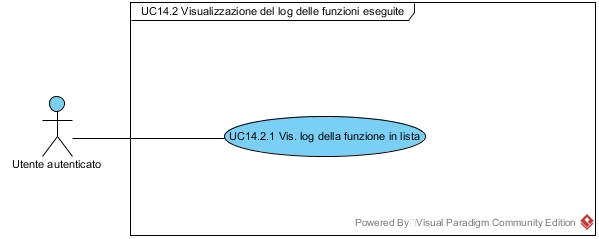
\includegraphics[width=0.7\linewidth]{res/img/UC14.2.jpg}
	\caption{Diagramma UC14.2 - Visualizzazione risultati del "list"}
\end{figure}
\begin{itemize}
	\item \textbf{Attori primari:} Utente autenticato;
	\item \textbf{Descrizione:} l'utente visualizzerà sul \textit{CLI\glo} il risultato del comando "list";
	\item \textbf{Pre-condizioni:} l'utente ha eseguito il comando "list";
	\item \textbf{Post-condizioni:} \textit{CLI\glo} visualizza l'elenco e le informazioni relative alle funzioni presenti nel sistema;
	\item \textbf{Scenario principale:} Il sistema mostrerà sulla \textit{CLI\glo} le informazioni relative a tutte le funzioni presenti su \textit{Etherless\glos}.
%    		\begin{itemize}
%    			\item autore;
%    			\item costo;
%    			\item descrizione;
%    			\item firma della funzione.
%    		\end{itemize}
\end{itemize}